\documentclass[a4paper, 11pt]{article}
\usepackage{comment}
\usepackage{lipsum} 
\usepackage{fullpage} %cambiar margen
\usepackage[a4paper, total={7in, 10in}]{geometry}

\usepackage{amssymb,amsthm} 
\usepackage{amsmath}
\newtheorem{theorem}{Theorem}
\newtheorem{corollary}{Corollary}
\usepackage{graphicx}
\usepackage{tikz}
\usetikzlibrary{arrows}
\usepackage{verbatim}
%\usepackage[numbered]{mcode}
\usepackage{float}
\usepackage{tikz}
\usetikzlibrary{shapes,arrows}
\usetikzlibrary{arrows,calc,positioning}
\usepackage{mathpazo} %tipo de letra 
\usepackage[utf8]{inputenc} %codificación
\usepackage[T1]{fontenc} %digitación de tildes y ñ
\usepackage[spanish]{babel} %paquete de soporte español

\tikzset{
	block/.style = {draw, rectangle,
		minimum height=1cm,
		minimum width=1.5cm},
	input/.style = {coordinate,node distance=1cm},
	output/.style = {coordinate,node distance=4cm},
	arrow/.style={draw, -latex,node distance=2cm},
	pinstyle/.style = {pin edge={latex-, black,node distance=2cm}},
	sum/.style = {draw, circle, node distance=1cm},
}
\usepackage{xcolor}
\usepackage{mdframed}
\usepackage[shortlabels]{enumitem}
\usepackage{indentfirst}
\usepackage{hyperref}

\usepackage{listings}
\lstset{literate=
  {á}{{\'a}}1
  {é}{{\'e}}1
  {í}{{\'i}}1
  {ó}{{\'o}}1
  {ú}{{\'u}}1
  {Á}{{\'A}}1
  {É}{{\'E}}1
  {Í}{{\'I}}1
  {Ó}{{\'O}}1
  {Ú}{{\'U}}1
  {ñ}{{\~n}}1
  {ü}{{\"u}}1
  {Ü}{{\"U}}1
}

\lstdefinestyle{customc}{
  belowcaptionskip=1\baselineskip,
  breaklines=true,
  frame=L,
  xleftmargin=\parindent,
  language=Python,
  showstringspaces=false,
  basicstyle=\footnotesize\ttfamily,
  keywordstyle=\bfseries\color{green!40!black},
  commentstyle=\itshape\color{purple!40!black},
  identifierstyle=\color{blue},
  stringstyle=\color{orange},
}

\lstdefinestyle{customasm}{
  belowcaptionskip=1\baselineskip,
  frame=L,
  xleftmargin=\parindent,
  language=[x86masm]Assembler,
  basicstyle=\footnotesize\ttfamily,
  commentstyle=\itshape\color{purple!40!black},
}

\lstset{escapechar=@,style=customc}



\renewcommand{\thesubsection}{\thesection.\alph{subsection}}

\newenvironment{problem}[2][Ejercicio]
{ \begin{mdframed}[backgroundcolor= red!50] \textbf{#1 #2} \\}
	{  \end{mdframed}}

% Define solution environment
\newenvironment{solution}
{\textcolor{blue}{\textbf{\textit{Solución:\\\noindent}}}}


\renewcommand{\qed}{\quad\qedsymbol}

% \\	
\begin{document}
	\noindent
	%%%%%%%%%%%%%%%%%%%%%%%%%%%%%%%%%%%%
	
	\begin{minipage}[b][1.2cm][t]{0.8\textwidth}
		\large\textbf{César Isaí García Cornejo} \hfill \textbf{Tarea 9}  \\
		cesar.cornejo@cimat.mx \hfill \\
		\normalsize Computo Científico \hfill Semestre 3\\
	\end{minipage}
	
	\hspace{14.4cm}
	\begin{minipage}[b][0.03cm][t]{0.12\linewidth}
		
		\vspace{-2.2cm}
		%%%La Ruta dependerá de donde este alojado el main y la imagen
		
\includegraphics[scale=0.3]{Figures/EscudoCimat.png}
	\end{minipage}
	
	\noindent\rule{7in}{2.8pt}
	
	%%%%%%%%%%%%%%%%%%%%%
	%%%%%%%%%%%%%%%%%%%%%%%%%%%%%%%%%%%%%%%%%%%%%%%%%%%%%%%%%%%%%%%%%%%%%%%%%%%%%%%%%%%%%%%%%%%%%%%%%%%%%%%%%%%%%%%%%%%
	% Problem 1
	%%%%%%%%%%%%%%%%%%%%%%%%%%%%%%%%%%%%%%%%%%%%%%%%%%%%%%%%%%%%%%%%%%%%%%%%%%%%%%%%%%%%%%%%%%%%%%%%%%%%%%%%%%%%%%%%%%%%%%%%%%%%%%%%%%%%%%%%
	\setlength{\parskip}{\medskipamount}
	\setlength{\parindent}{0pt}
%/////////// Ejercicio 1 /////////////////

\begin{problem}{1} 
    En ambos problemas hay que diseñar e implementar el MCMC, investigar sobre su convergencia y tener algún grado de certeza si sí se está simulando de la posterior correspondiente. Más aún, recuerde que se trata de un problema de inferencia. Hay que hablar del problema en si, comentar sobre las posteriores simuladas y posibles estimadores ( a partir de la muestra de posterior) que se puede proporcionar de cada parámetro.
\end{problem}

\begin{problem}{(Problema en ecología)} 
    Sean $X_1, ..., X_m$ variables aleatorias donde $X_i$ denota el número de individuos de una especie en cierta región. Suponga que $X_i|N,p\sim Binomial(N,p)$, entonces 
    \begin{align*}
        f(\bar{X}|N,p) = \prod_{i = 1}^{m} \frac{N!}{x_i!(N-x_i)!} p^{x_i}(1-p)^{N-x_i}.
    \end{align*}
    Asumiendo la distribución a priori $p\sim Beta(\alpha,\beta)$ y $N\sim h(\cdot)$, donde $h$ es una dist. discreta en $\{0,1,2,...,N_{max}\}$, se tiene definida la distribución posterior $f(N,P|\bar{x})$.
    A partir del algoritmo MH, simule valores de a distribución posterior usando un kernel híbirido. Para ello considere como sugerencia la siguiente distribución inicial para el MCMC 
    \begin{align*}
        p \sim U(0,1)   \:\:\:\: y \:\:\:\: N\sim U_d \left \{  \max_{i\in \{1,...,m\} } (x_i), \max_{i\in \{1,...,m\} } (x_i) + 1, ..., N_{max} \right \}
    \end{align*}
    y las propuestas
    \begin{enumerate}
        \item Propuesta 1: De la condicional total de p (kener Gibbs).
        \item Propuesta 2: De la a priori
        \item Propuesta 3: Propuesta hipergeométrica
        \item Propuesta 4: Poisson: $N_p \sim \max_{i \in \{1,...,m\} }(x_i) + Poisson(\cdot)$.
        \item Propuesta 5: Caminata aleatoria 
        \begin{align*}
            N_p = N + \varepsilon, \:\:\:\: \mathbb{P}\left (\varepsilon = 1 \right ) = \frac{1}{2} = \mathbb{P}\left (\varepsilon = -1 \right )    
        \end{align*}
    \end{enumerate}
    Los datos son estos: 7,7,8,8,9,4,7,5,5,6,9,8,11,7,5,5,7,3,10,3.

    A priori, esperamos que sea difícil observar a los individuos entonces $\alpha = 1, \beta = 20$ . La especie no es muy abundadnte y entonces $N_{max} = 1000$ y $h(N) = 1/(N_{max} +1); N \in \{0,1,2,...,N_{max}\}$.
    Las propuestas y distribución inicial para el MCMC de arriba son solamente sugerencia, propongan otras propuestas, experimente y comenten.
\end{problem}
    

\begin{solution} 
    

    Tenemos un grupo de individuos que se modelan según una ley binomial para cierta región. Luego, desconocemos los parámetros de dicha ley. Con la metodología dada por la inferencia bayesiana, se propone cada parámetro como una variable aleatoria y aplicamos la metodología usual para determinar la distribución a posterior, que es la distribución de los parámetros dadas las observaciones. Como establece el enunciado, las distribuciones a priori se propusieron como beta y uniforme discreta, respectivamente. 

    La función objetivo es en nuestro caso la distribución a posteriori, cuya expresión explícita es 
    \begin{align*}
        f(p, N ) &\propto \mathcal{L} (p,N|\bar{x}) f(p,N) \\
        &\propto \left( \prod_{i = 1}^{m} \frac{N!}{x_i!(N-x_i!)} p ^{x_i} (1-p_i)^{N-x_i}\right) \cdot p^{\alpha-1}(1-p)^{\beta -1} \cdot \frac{1}{N_{max} + 1}  \mathbb{1}_{\{0,1,...,N_{max}\}} (N)
    \end{align*}
    Se pueden quitar ciertas constantes y reacomodar la expresión para obtener la expresión simplificada. Sin embargo, como es usual, y por estabilidad numérica buscamos el logaritmo de la objetivo obteniendo
    \begin{align*}
        \log f(p,N|\bar{x})  \propto &  \: m \log(N!) - \sum \log x_i! - \sum \log(N-x_i)! + \sum x_i \log p + \\ + & (mN- \sum x_i)\log(1-p) + (\alpha - 1) \log p + (\beta -1 )\log (1-p)
    \end{align*}

    Se proponen los puntos iniciales tal como es sugerido con el siguiente comando
    \begin{lstlisting}
    N_max = 1000
    w = np.arange(max(x)+ 1, N_max)

    p_0 = uniform.rvs(0,1)
    N_0 = random.choice(w)
    \end{lstlisting}

    Notemos que para simular de una uniforme discreta se uso random.choice que selecciona al azar de un elemento en la lista previamente definida.

    Se define cada propuesta, para tomar de forma equiprobable con kerneles híbridos. La primer propuesta solo salta de valores en $p$ y mantiene $N$ constante, está ayuda a bajar los valores altos de $N$ en la siguiente iteración. La segunda propuesta por si sola es suficiente ya que con ella se obtendría gráficas parecidas a la obtenida con el kernel híbrido. La tercer y cuarta propuesta se parecen en el sentido de que se agrega una cantidad no nula, solamente hay que cuidar que no supere a $N_{max}$, ambas aumentan el valor de $N$. Por último la quinta propuesta es una caminata aleatoria sobre $N$ que también aumenta su valor a la vez que lo disminuye. 
    
    Luego, con el método de Metropolis-Hastings tenemos una realización de la trayectoria que se muestra a continuación
    \begin{figure}[H] 
        \centering 
        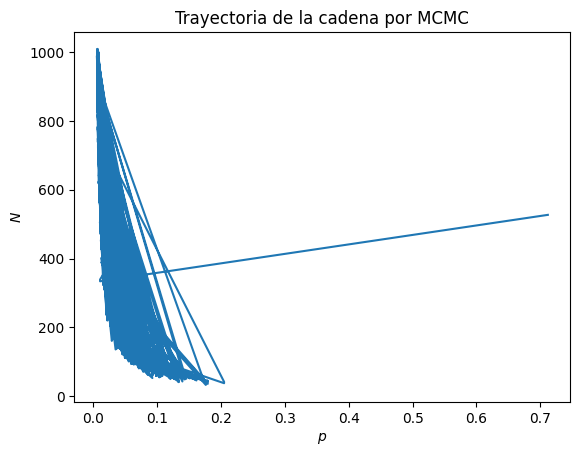
\includegraphics[width = 10 cm]{Figures/trayectoria.png} 
        \caption{Trayectoria de la cadena por MCMC.}
        \label{Fig. 9.01}
    \end{figure} 
    Vemos que tenemos un salto pronunciado, esto se debe al punto inicial que es tomado al azar en cualquier parte del recuadro. Veamos de que tamaño necesita ser el burn-in para que se consideren el resto de las simulaciones como muestras de la función objetivo. 

    Graficamos la evolución de la cadena para cada iteración obteniendo 
    \begin{figure}[H] 
        \centering 
        \includegraphics[width = 10 cm ]{Figures/evolución.png} 
        \caption{Evolución de la cadena para las primeras 4000 iteraciones.}
        \label{Fig. 9.02}
    \end{figure} 

    Notamos que para la variable $p$ tenemos una disparidad, considerable del valor inicial con los posteriores. En contraste, dicha disparidad no ocurre para $N$. Como la cadena empieza relativamente cerca a su distribución convergente, entonces podemos tomar un burn in no muy grande. Para nuestro propósito $n = 1000$ es suficiente. 

    La trayectoria de las simulaciones con burn in es ahora 
    \begin{figure}[H] 
        \centering 
        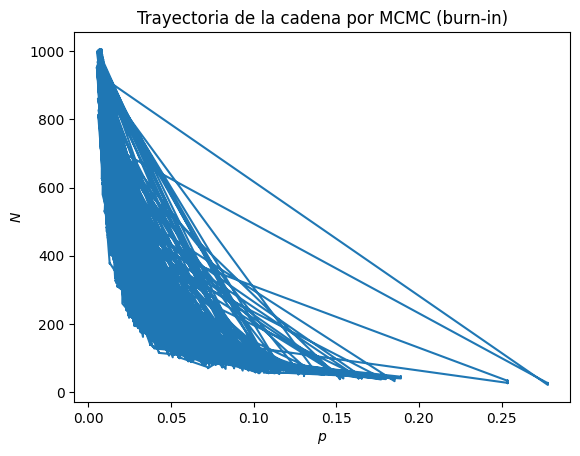
\includegraphics[width = 10 cm]{Figures/trayectoria_burn.png} 
        \caption{Trayectoria de la cadena por MCMC con burn-in.}
        \label{Fig. 9.03}
    \end{figure} 
    Notemos que se limpia la trayectoria inicial con un cambio abrupto. Luego, obtenemos los histograma de las distribuciones marginales.
    \begin{figure}[H] 
        \centering 
        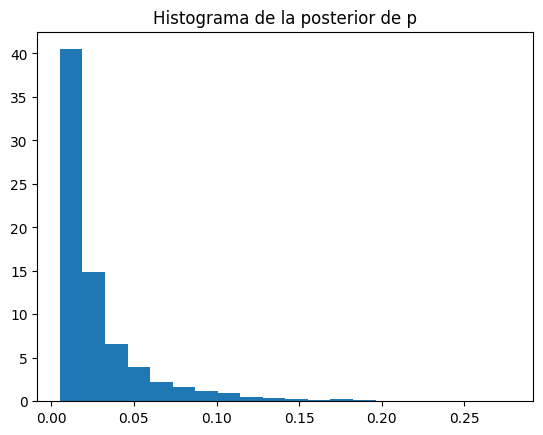
\includegraphics[width = 10 cm]{Figures/p.png} 
        \caption{Histograma para la distribución posterior de $p$.}
        \label{Fig. 9.04}
    \end{figure} 
    y el histograma para $M$ es
    \begin{figure}[H] 
        \centering 
        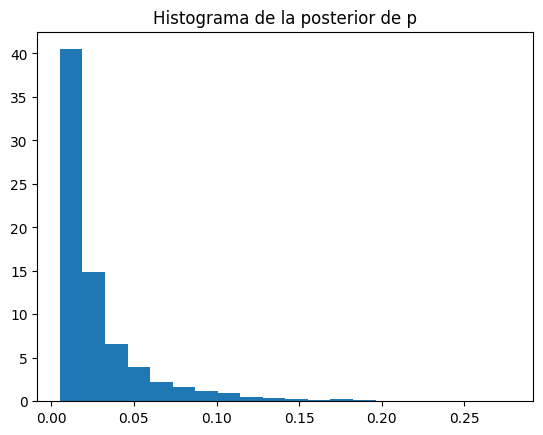
\includegraphics[width = 10 cm]{Figures/p.png} 
        \caption{Histograma para la distribución posterior de $p$.}
        \label{Fig. 9.05}
    \end{figure} 


    Para obtener una estimación puntual de los parámetros, con el estimador de bayes muestral obtenemos la media de las simulaciones dando:
    \begin{lstlisting}
Media muestral para p:  0.027603744890256174
Media muestral para N: 448.74062
    \end{lstlisting}
    que nos deja la estimación bayesiana del modelo y concluye el ejercicio.













\end{solution}
\newpage

\begin{problem}{(Estudio de mercado)} 
    Se tiene un producto y se realiza una encuesta con el fin de estudiar cuánto se consume dependiendo de la edad. Sea $Y_i$ el monto de compra y $X_i$ la covariable la cuál representa la edad. Sea $Y_i$ el monto de compra y $X_i$ la covariable la cual representa la edad. 

    Suponga que $Y_i \sim Po(\lambda_i)$ 
    \begin{align*}
        \lambda_i  = cg _b(x_i -a)
    \end{align*}
    para $g_b$ la siguiente función  de liga
    \begin{align*}
        g_b(x) = \exp \left(-\frac{-x^2}{2b^2}  \right) 
    \end{align*}
    O sea, se trata de regresión Poisson con una función de liga no usual. Si $\lambda_i = 0$ entonces $\mathbb{P}\left (Y_i = 0 \right ) = 1. $a = años  medios del segmento (años), c = gastos promedio (pesos), b = `amplitud' del segmento (años). 

    Considere la distribución a priori 
    \begin{align*}
        \alpha \sim N(35, 5) , \:\:\:\: c \sim Gama(3,3/350) \:\:\:\: b \sim Gama(2,2/5).
    \end{align*}

    El segundo parámetro  de la normal es la desviación estándar y el segundo parámetro de las gamas es la taza.

    Usando MH simule de la distribución posterior de a, c y b.
    Los datos son estos n= 100.


\end{problem}

\begin{solution} 
    
\end{solution}

\begin{problem}{3} 
    Investiga y describe brevemente los softwares OpenBugs, Nimble, JAGS, DRAM, Rtwalk, Mcee Hammer, PyMCMC.
\end{problem}

\begin{solution} 
    OpenBUGS

    Es un software libre utilizado para análisis estadístico, específicamente para modelos bayesianos. Tiene funcionalidades avanzadas para el muestreo MCMC y puede ejecutarse de forma nativa en Linux. En este se pueden definir modelos estadísticos utilizando una notación similar a la de un modelo probabilístico y utiliza métodos de muestro de Monte Carlo y Gibbs para aproximar la distribución posterior. Otra ventaja es que se puede utilizar mediante lenguajes como R y Python, entre otros. 
    
    Por ejemplo, si se quiere usar en Python, se debe de importar “pybugs”, y escribir el modelo en formato BUGS, después se definen los parámetros, se crea una instancia y finalmente se realiza el muestreo.
    
    NIMBLE
    
    La sigla NIMBLE proviene de “Numerical Inference for Statistical Models Using Bayesian and Likehood Estimation”. Es una paquetería para construir y compartir modelos estadísticos. Facilita la programación de algoritmos estadísticos, es una extensión de BUGS y también se puede entender como una biblioteca de algoritmos como MCMC. 
    Para ejecutar nimble en R, se debe de usar la paquetería “nimble”, definir el modelo, crear un modelo con “nimbleModel”, compilarlo y hacer el muestreo de Gibbs para inferencia bayesiana con “MCMC”. 
    
    JAGS
    La sigla JAGS significa “Just Another Gibbs Sampler” es un programa para el análisis jerárquico bayesiano que utiliza la simulación MCMC no tan distinta a BUGS.  Es un software que permite especificar modelos estadísticos en un formato similar al lenguaje BUGS, lo que hace que sea sencillo definir los modelos. Algunas características son: especificación del modelo similar a BUGS, implementación de muestreo de Gibbs, puede utilizarse para modelos bayesianos simples o complejos, se puede utilizar en R, Python, matlab, entre otros. 
    
    Para utilizarlo en R, se debe de instalar “rjags” y después sigue un procedimiento similar a los ya mencionados. 
    
    DRAM
    Significa “Delayed Rejection Adaptive Metropolis”, es un método de optimización utilizado para el MCMC. Se usa específicamente para mejorar la eficiencia y la capacidad de exploración del espacio de parámetros. Se basa en el método Metropolis-Hastings, y su idea principal es la introducción de mecanismos de rechazo diferido para mejorar la eficiencia de adaptación; esto permite realizar múltiples intentos para generar una muestra aceptable. 
    Para usar este método se debe de instalar “MCMCpack”, y para ejecutar DRAM se utiliza la función “MCMCmetrop1R”. 
    
    Rtwalk 
    Es un algoritmo de simulación utilizado para MCMC. Se usa para explorar y muestrear de forma eficiente el espacio de parámetros. Este método realiza pasos en el espacio de parámetros basándose en una caminata aleatoria para explorar diferentes regiones y capturar muestras representativas de la distribución. Es un algoritmo adaptable, y con ello mejora la eficiencia de la exploración. 
    
    No es un algoritmo estándar en R, pero se puede hacer a partir de generar muestras de una función objetivo, realizar pasos aleatorios y aceptando o rechazando los pasos. 
    
    The MCMC Hammer
    Es una herramienta introducida por la comunidad astronómica. Está diseñada para implementar el algoritmo MCMC, para realizar inferencia bayesiana y estimación de parámetros astronómicos complejos. 
    
    PyMCMC
    Ahora llamado “PyMC” es un módulo de Python que implementa estadística Bayesiana incluida MCMC. Incluye un gran conjunto de distribuciones estadísticas, utiliza Numpy para lo numérico, utiliza un modulo para modelar procesos Gausianos, puede hacer resúmenes, también hay muchos diagnósticos de convergencia, etcétera. 
    Para usarlo se debe de importar “pymc” y utilizar funciones tipo “pymc.Normal, pymc.Binomial”. 
     
\end{solution}


\begin{thebibliography}{9}

    \bibitem{Casella}
    Robert, C. P., Casella, G., and Casella, G. (1999). Monte Carlo statistical methods (Vol. 2). New York: Springer.

    \bibitem{Wasserman}
    Wasserman, L. (2004). All of statistics: a concise course in statistical inference (p. 413). New York: Springer.
    
\end{thebibliography}
      




\end{document}